\section{Техническое задание}
\subsection{Основание для разработки}

Основанием для разработки является задание на выпускную квалификационную работу бакалавра "<Веб-приложение для компьютерной поддержки самостоятельной работы  иностранных студентов при изучении языка программирования  JavaScript">.

\subsection{Цель и назначение разработки}

Основной задачей выпускной квалификационной работы является разработка и внедрение веб-приложения для компьютерной поддержки самостоятельной работы  иностранных студентов при изучении языка программирования  JavaScript.

Посредством внедрения веб-приложения планируется устранить существующие недостатки, связанные с неструктурированным доступом к учебным материалам, отсутствием интерактивных инструментов для практики и тестирования, а также сложностями в организации учебного процесса для иностранных студентов, включая языковые барьеры.

Цель разработки включает следующие подцели:

\begin{itemize}
\item создание единой образовательной платформы для доступа к учебным курсам, урокам и тестам;
\item обеспечение удобного и интуитивно понятного интерфейса для самостоятельного изучения JavaScript;
\item интеграция инструментов для проверки знаний, таких как тесты с автоматической оценкой;
\item оптимизация процессов управления учебным контентом для преподавателей и взаимодействия студентов с платформой.
\end{itemize}

\subsection{Функциональные задачи}

Разрабатываемая веб-платформа включает в себя следующие модули:
\begin{enumerate}
\item \textbf{Курсы} — модуль для создания и управления учебными курсами, включающими уроки и тесты. Преподаватели могут добавлять, редактировать и удалять курсы, а студенты получают доступ к материалам.;
\item \textbf{Уроки} — система управления учебным контентом, позволяющая структурировать материалы курса (текст, изображения, видео) и задавать порядок уроков. Поддерживается предпросмотр уроков и их редактирование.;
\item \textbf{Тесты} — модуль для создания и прохождения интерактивных тестов. Преподаватели могут задавать вопросы и варианты ответов, а студенты проходят тесты с автоматической оценкой результатов;
\item \textbf{Результаты тестов} — инструмент для анализа успеваемости студентов. Преподаватели могут просматривать, удалять и управлять результатами тестов, включая статистику по студентам;
\item \textbf{Панель управления преподавателя} — интерфейс для управления курсами, уроками, тестами и результатами, с удобной навигацией и виджетами для быстрого доступа;
\item \textbf{Профиль пользователя} — модуль для управления учетной записью, включая настройки аватара и персональной информации;
\item \textbf{Сообщения} — система уведомлений для обратной связи (например, сообщения об успешном добавлении урока или удалении результатов);
\item \textbf{Панель управления} — страница с виджетами всех вышеперечисленных сервисов.
\end{enumerate}

\subsection{Требования пользователя к интерфейсу web-сайта}

Платформа должна обеспечивать:
\begin{itemize}
    \item авторизацию;
    \item интуитивно понятную навигацию между модулями;
    \item адаптивный интерфейс для десктопных и мобильных устройств.
\end{itemize}

Композиция интерфейса пользователя представлена на рисунках ~\ref{templ:image1}, ~\ref{templ:image2}, ~\ref{templ:image3}, ~\ref{templ:image4}, ~\ref{templ:image5}, ~\ref{templ:image6}, ~\ref{templ:image7}, ~\ref{templ:image8}, ~\ref{templ:image9},  ~\ref{templ:image10}.
\newpage  

\subsection*{Композиция шаблона курсы представлена на рисунке ~\ref{templ:image1} и состоит из:}

\begin{itemize}
	\item кнопка для просмотра курса (1);
	\item окна с информацией роли профиля и имени (2);
	\item кнопка для создания курса (3);
	\item кнопка для просмотра своих курсов (4);
	\item кнопка для выхода (5);
	\item кнопка для смены языка (6).
\end{itemize}

\begin{figure}[htp!]
	\centering
	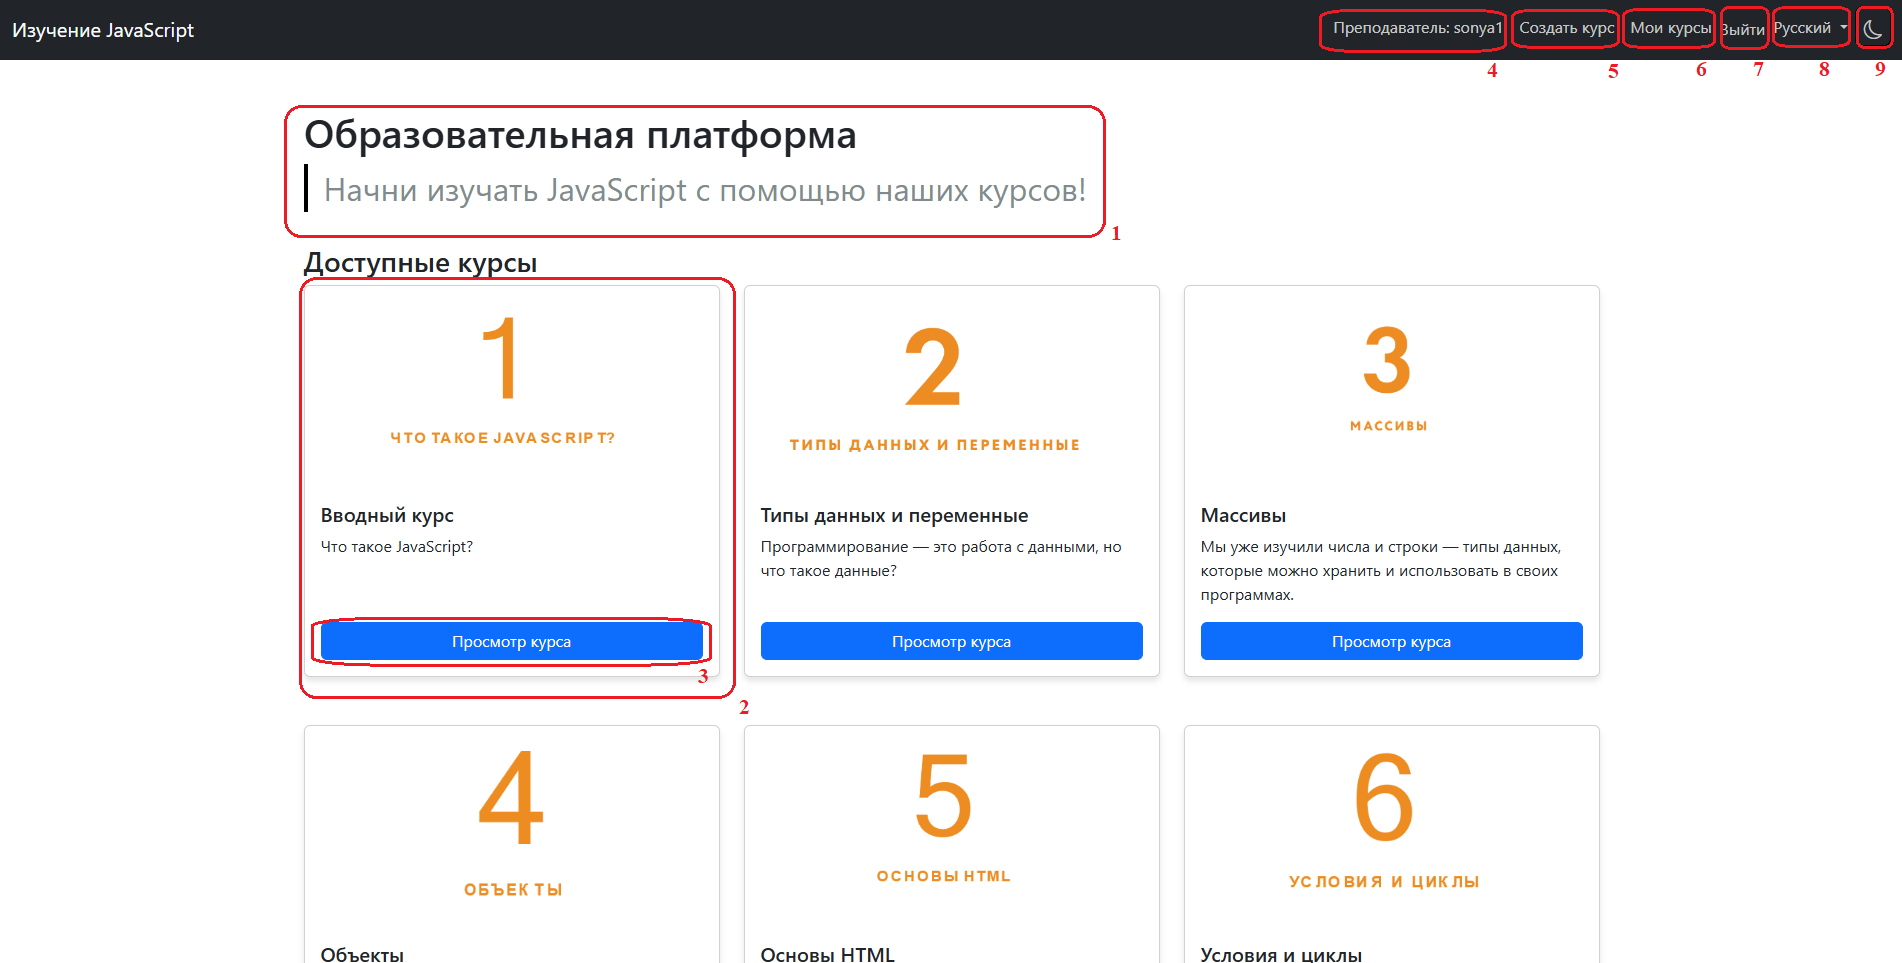
\includegraphics[width=0.7\linewidth]{images/курсы}
	\caption{Композиция интерфейса сервиса <<Курсы>>}
	\label{templ:image1}
\end{figure}

\subsection*{Композиция шаблона панель управления преподавателя представлена на рисунке ~\ref{templ:image2} и состоит из:}

\begin{itemize}
	\item кнопка для редактирования курса (1);
	\item кнопка для управления уроками (2);
	\item кнопка для просмотра курса (3);
	\item кнопка для удаления курса (4).
\end{itemize}

\begin{figure}[htp!]
	\centering
	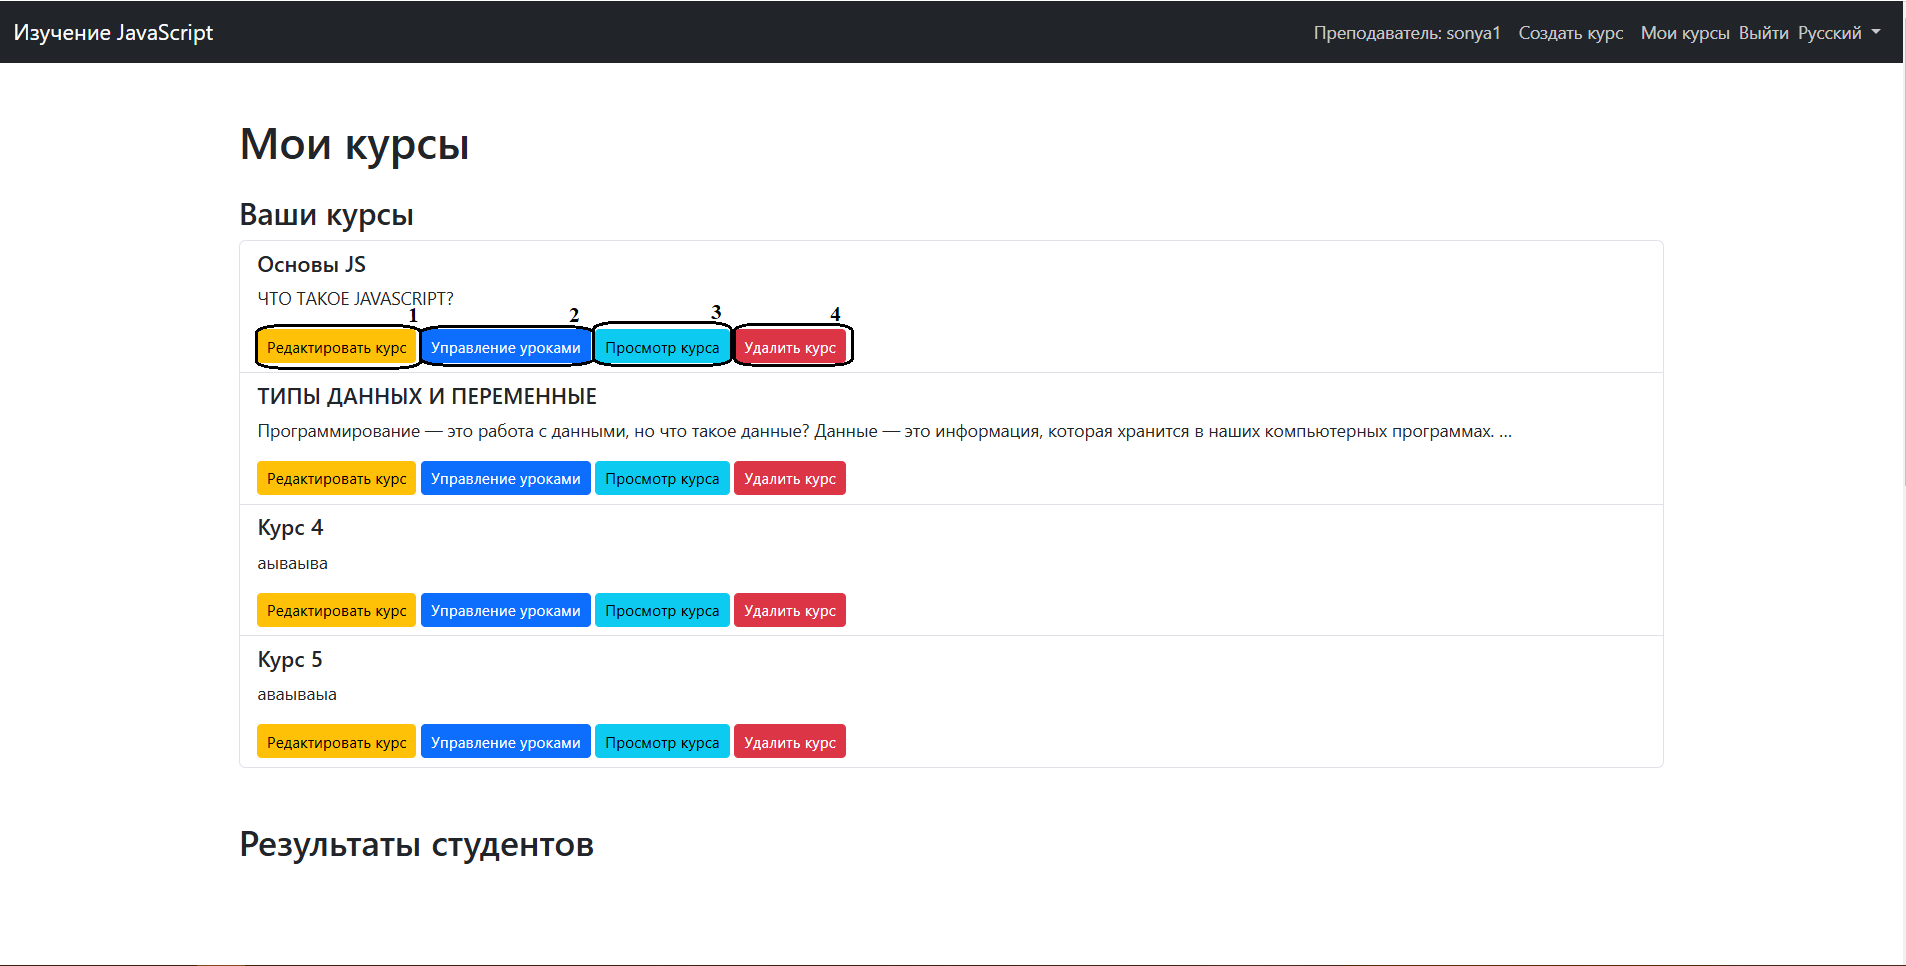
\includegraphics[width=0.7\linewidth]{images/учитель}
	\caption{Композиция интерфейса сервиса <<Панель управления преподавателя>>}
	\label{templ:image2}
\end{figure}
\newpage 
\subsection*{Композиция шаблона уроки представлена на рисунке ~\ref{templ:image3} и состоит из:}

\begin{itemize}
	\item кнопка для просмотра урока (1);
	\item окна курса (2);
	\item окно уроков (3);
	\item навигационная панель (4).
\end{itemize}

\begin{figure}[htp!]
	\centering
	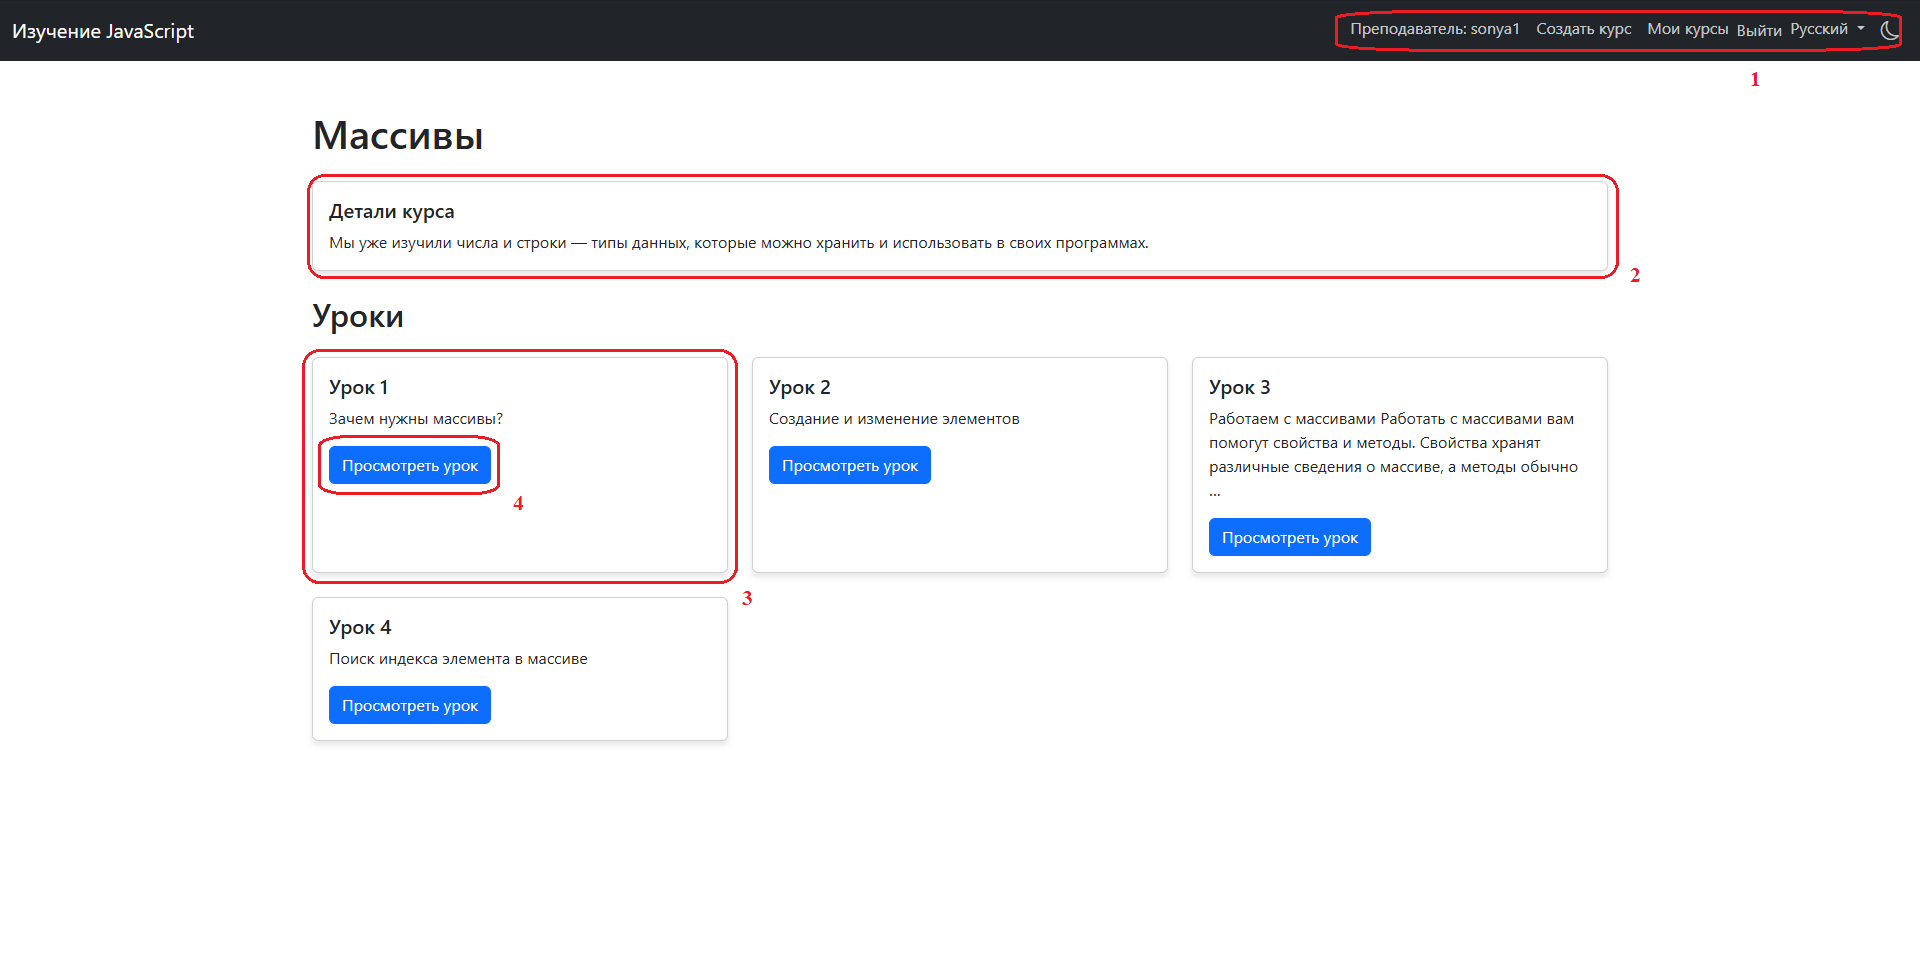
\includegraphics[width=0.8\linewidth]{images/уроки}
	\caption{Композиция интерфейса сервиса <<Уроки>>}
	\label{templ:image3}
\end{figure}

\subsection*{Композиция шаблона тесты представлена на рисунке ~\ref{templ:image4} и состоит из:}

\begin{itemize}
	\item окно уроков (1);
	\item кнопка редактировать урок (2);
	\item кнопка просмотр урока (3);
	\item кнопка обложка урока (4);
	\item кнопка добавить тест (5);
	\item кнопка управление вопросами (6);
	\item кнопка управление результатами (7).
\end{itemize}

\begin{figure}[htp!]
	\centering
	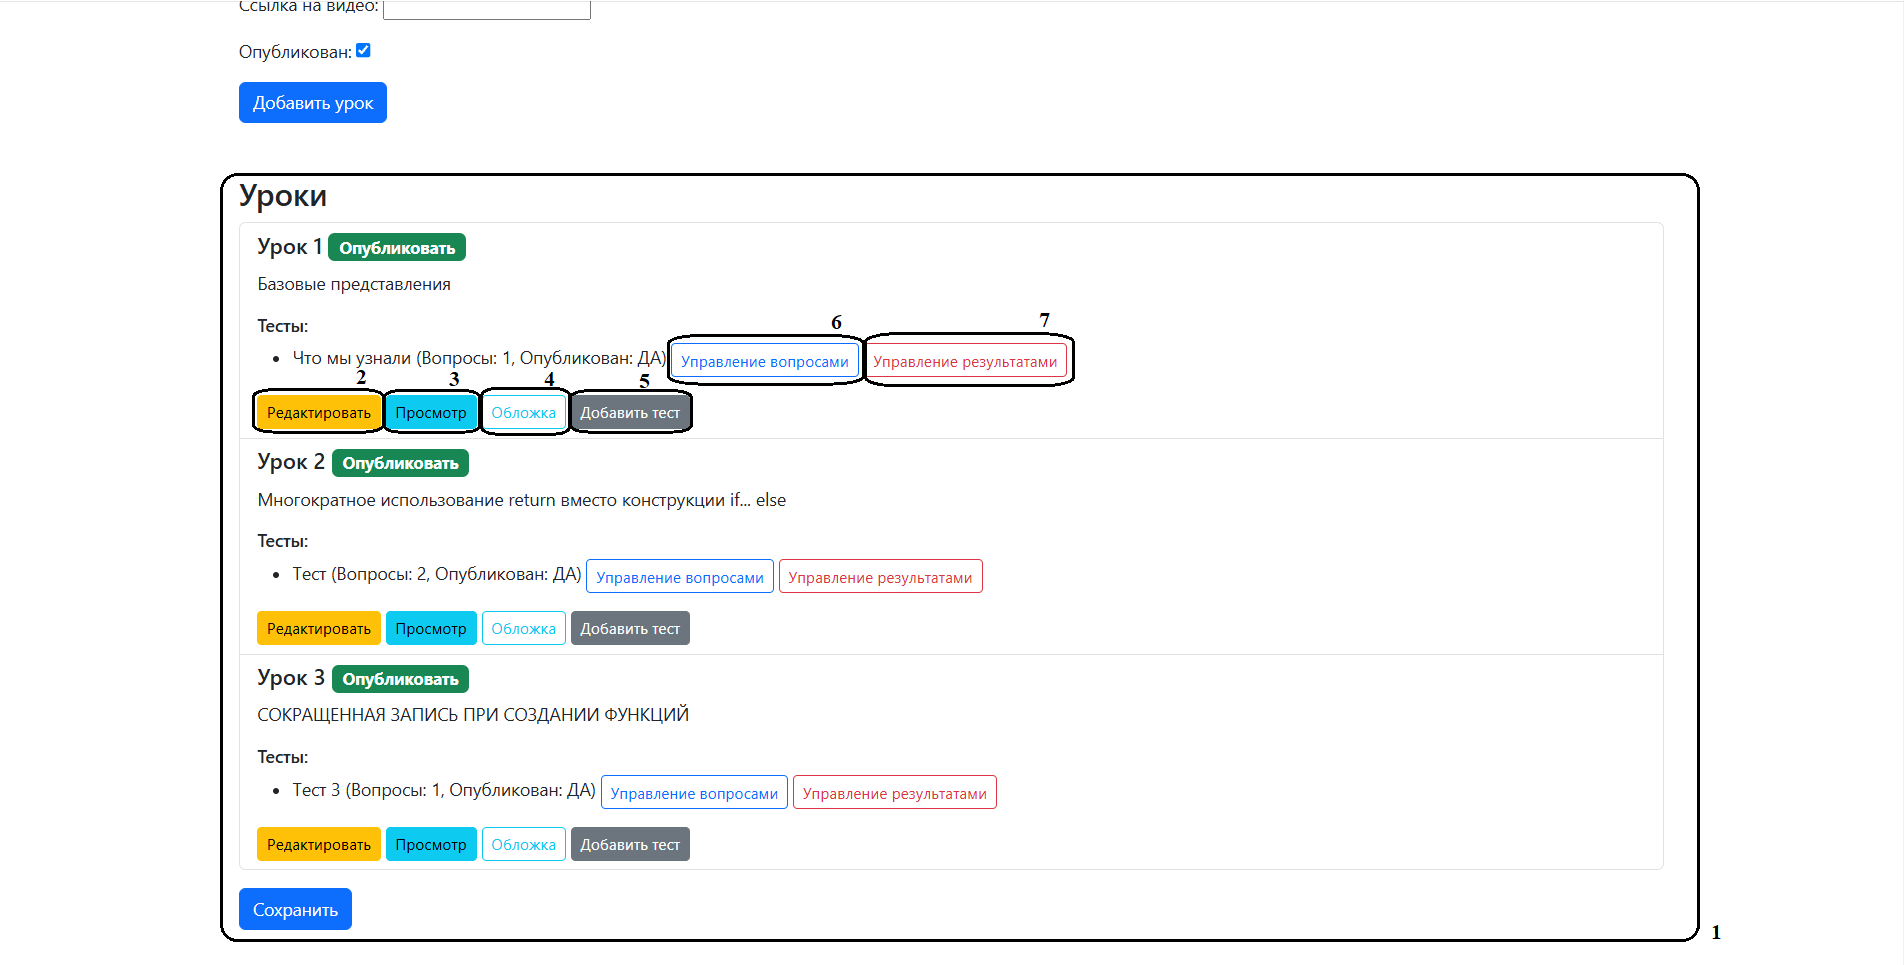
\includegraphics[width=0.8\linewidth]{images/Тесты}
	\caption{Композиция интерфейса сервиса <<Тесты>>}
	\label{templ:image4}
\end{figure}

\subsection*{Композиция шаблона создание теста представлена на рисунке ~\ref{templ:image5} и состоит из:}

\begin{itemize}
	\item окно создания теста (1);
	\item поле ввода заголовка теста (2);
	\item поле ввода описания теста (3);
	\item поле ввода минимального балла (4);
	\item поле выбора статуса (5);
	\item кнопка для создания теста (6);
	\item кнопка возвращения к уроку (7).
\end{itemize}

\begin{figure}[htp!]
	\centering
	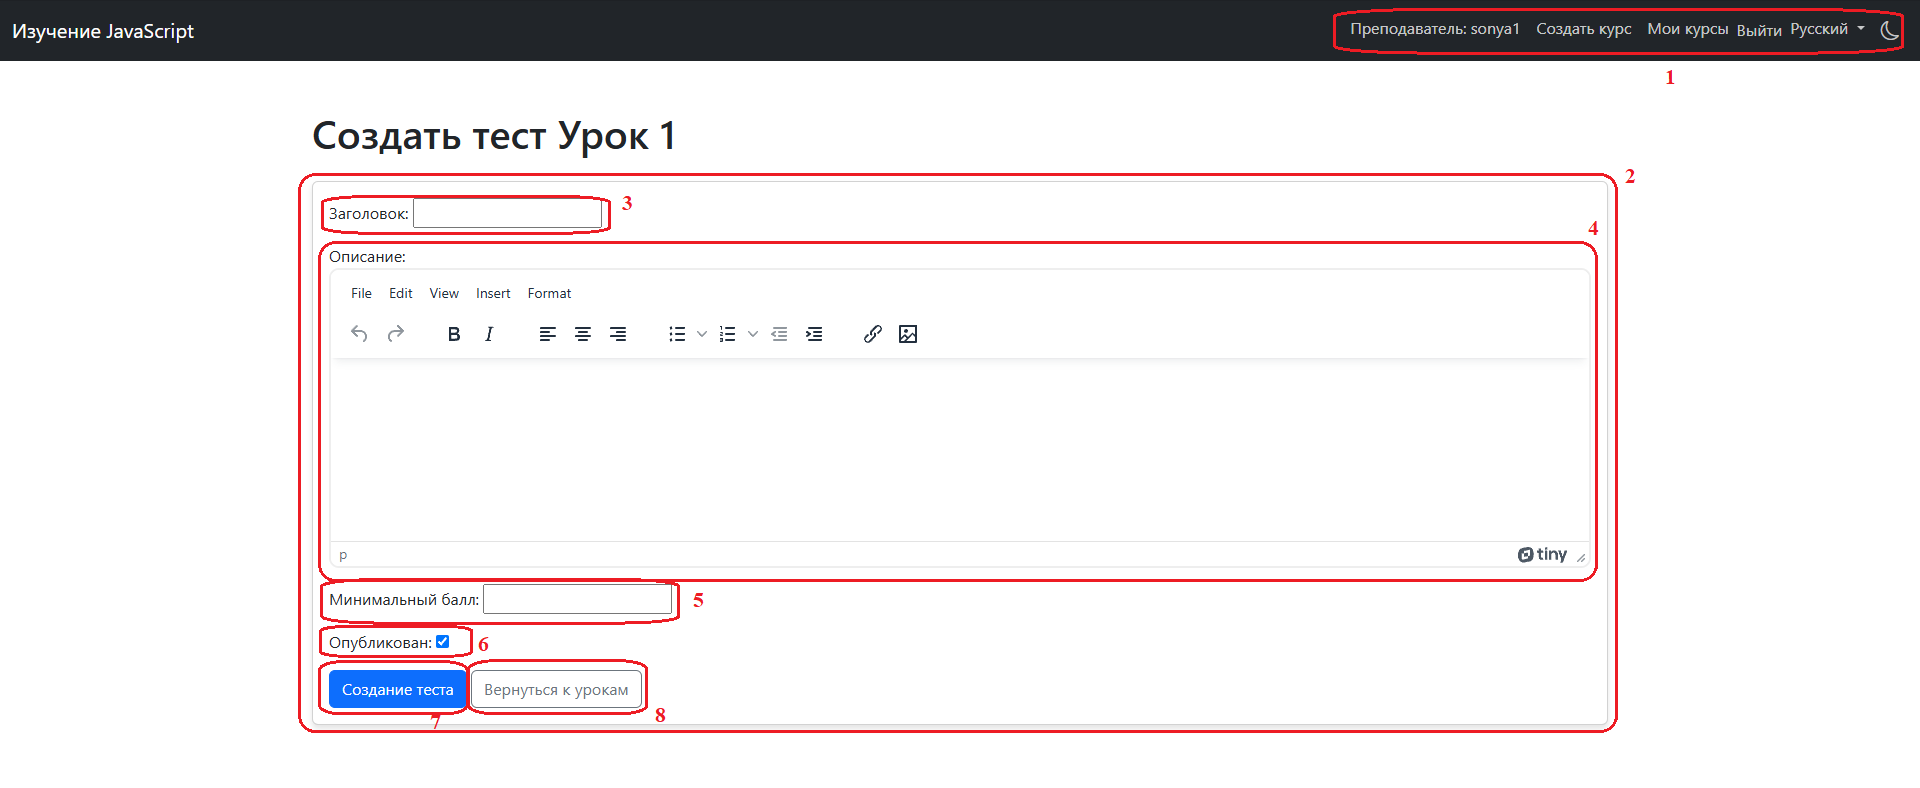
\includegraphics[width=0.8\linewidth]{images/создатьтест}
	\caption{Композиция интерфейса сервиса <<Создание теста>>}
	\label{templ:image5}
\end{figure}
\newpage
\subsection*{Композиция шаблона результаты теста представлена на рисунке ~\ref{templ:image6} и состоит из:}

\begin{itemize}
	\item окна управления результатами теста (1);
	\item окна с результатами студентов  (2);
	\item кнопка удалить все результаты (3);
	\item кнопка удалить результат (4);
	\item кнопка вернуться к вопросам (5);
	\item кнопка вернуться к урокам (6).
\end{itemize}

\begin{figure}[htp!]
	\centering
	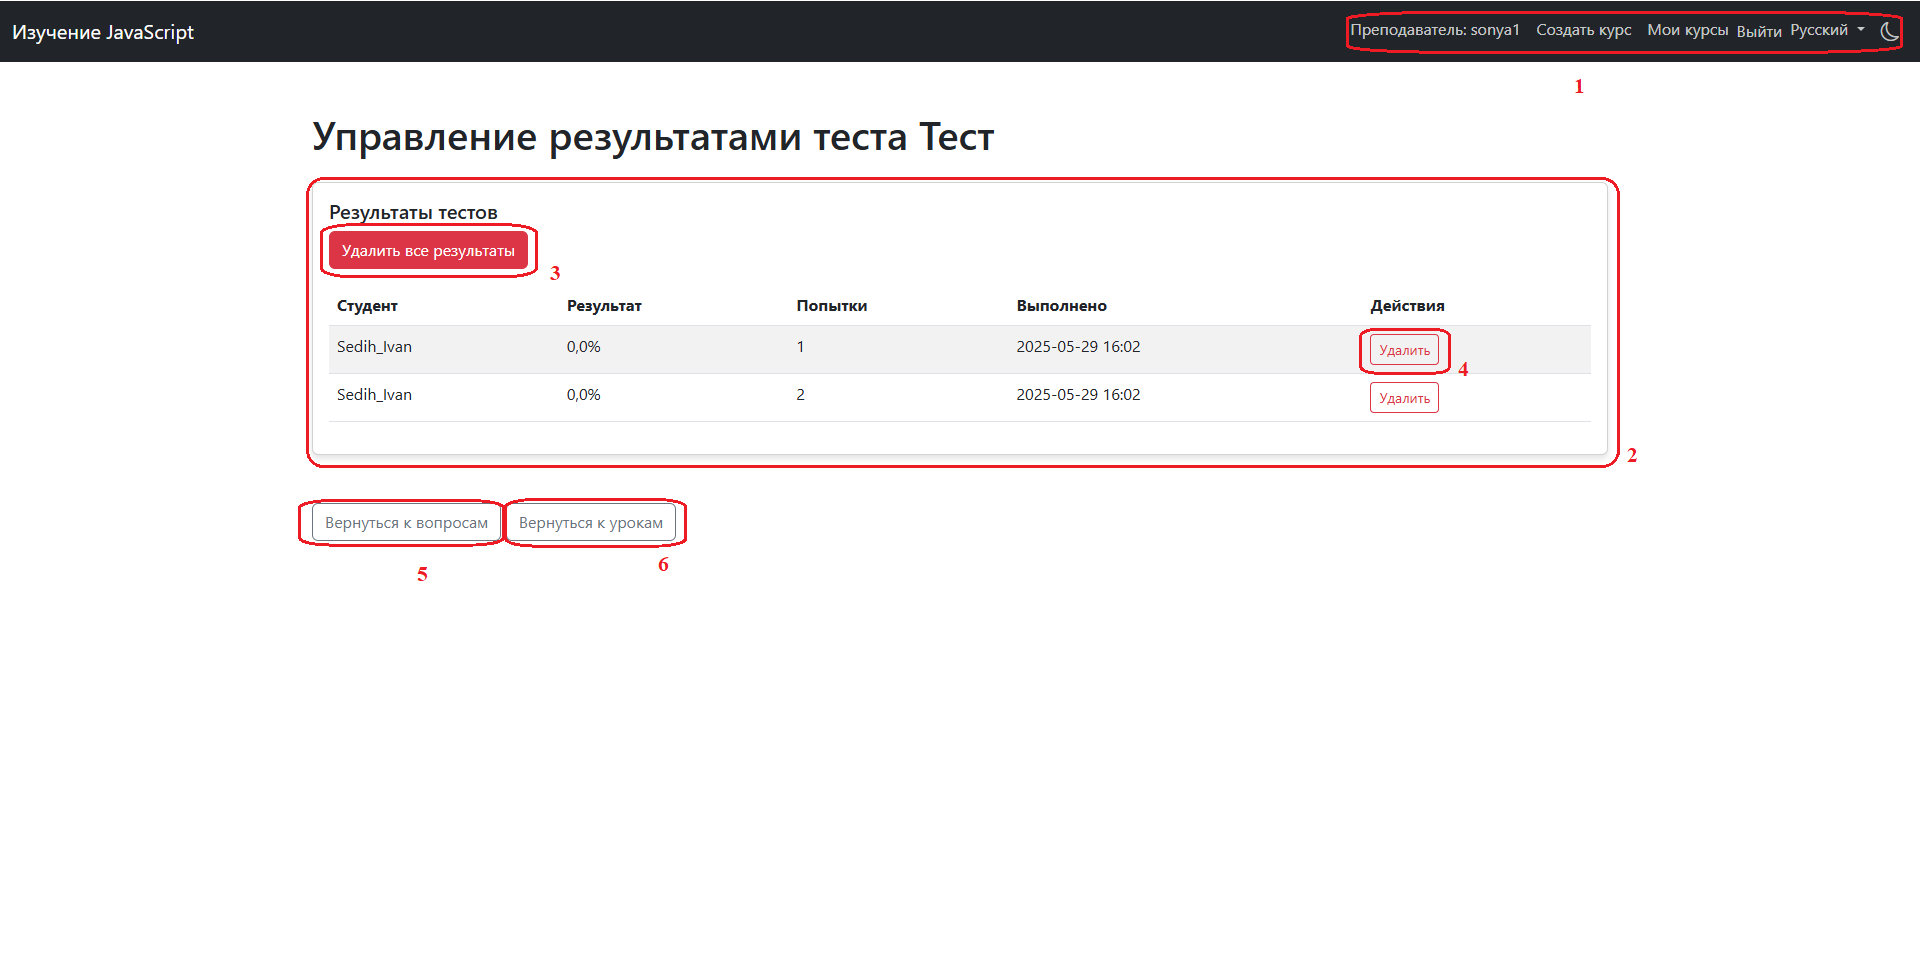
\includegraphics[width=0.8\linewidth]{images/результаты}
	\caption{Композиция интерфейса сервиса <<Результаты тестов>>}
	\label{templ:image6}
\end{figure}

\subsection*{Композиция шаблона окна авторизации представлена на рисунке ~\ref{templ:image7} и состоит из:}

\begin{itemize}
	\item поле для ввода кода (1);
	\item экранная клавиатура (2);
	\item кнопка для очистки поля (3);
	\item кнопка для подтверждения ввода пароля (4).
\end{itemize}

\begin{figure}[htp!]
	\centering
	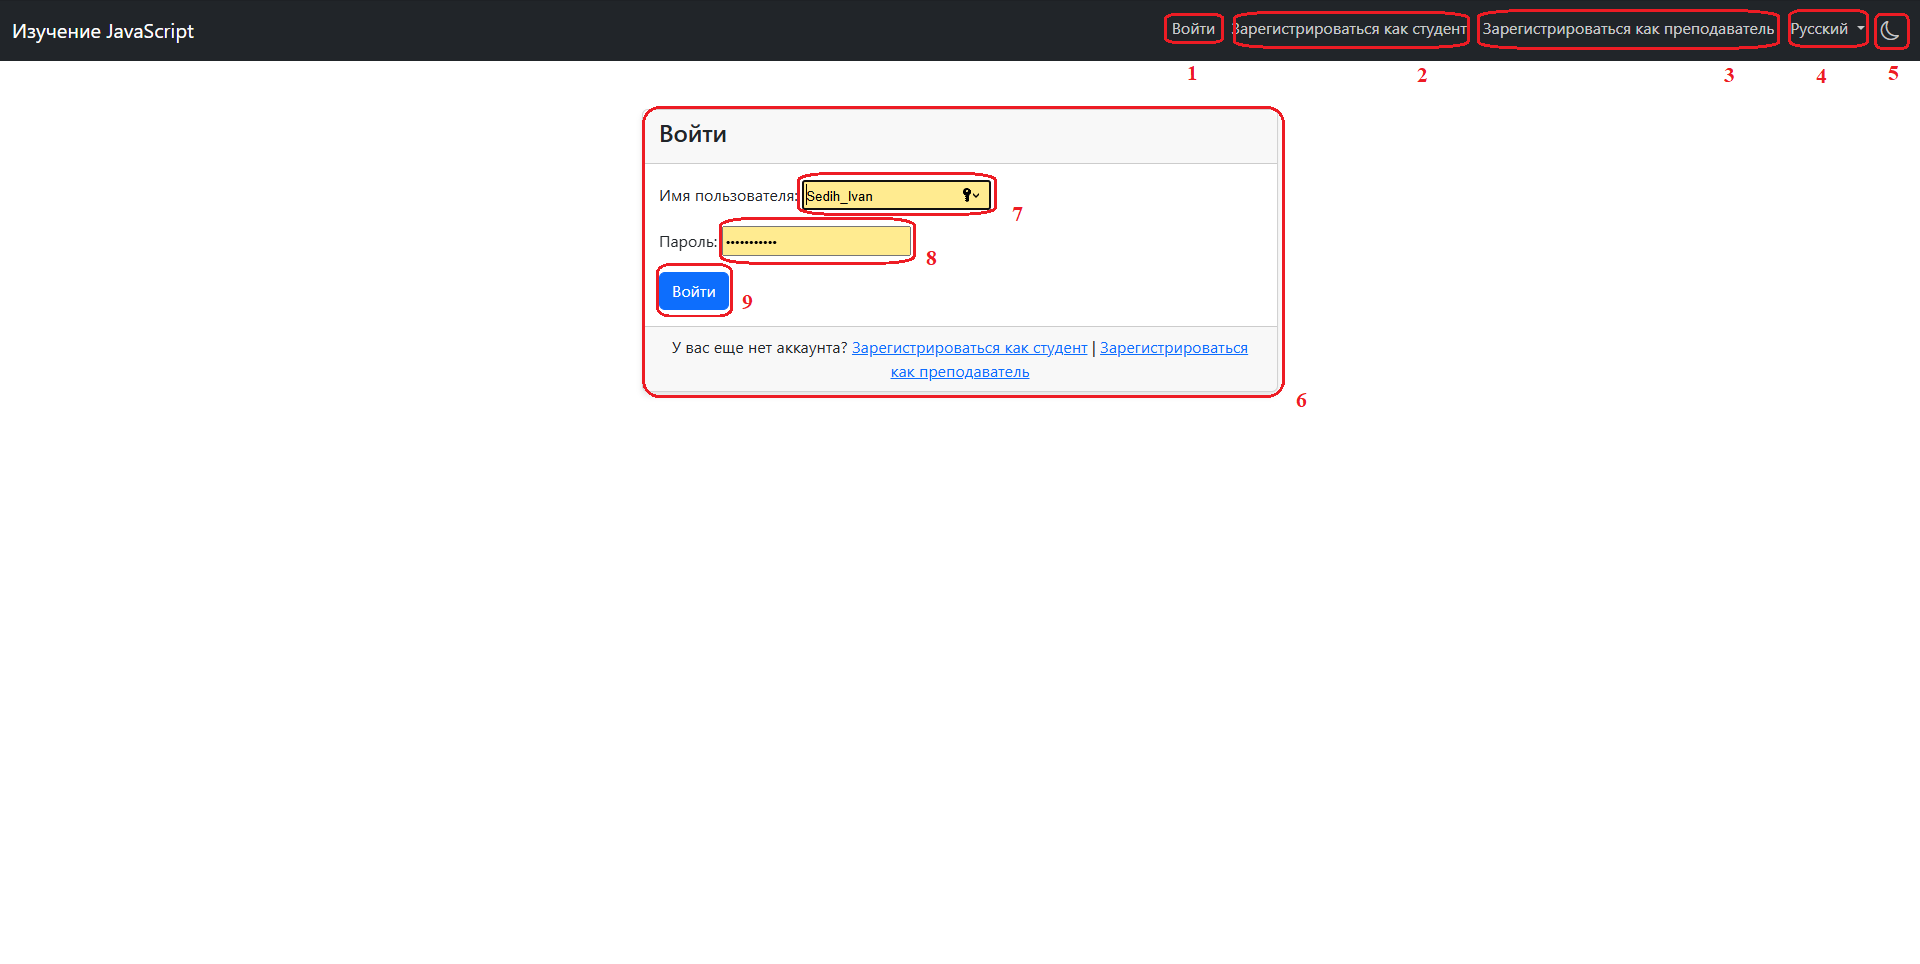
\includegraphics[width=0.8\linewidth]{images/Авторизация}
	\caption{Композиция интерфейса сервиса <<Авторизация>>}
	\label{templ:image7}
\end{figure}

\subsection*{Композиция шаблона профиль представлена на рисунке ~\ref{templ:image8} и состоит из:}

\begin{itemize}
	\item окно курсов на которые записан (1);
	\item кнопка просмотра курса (2);
	\item кнопка отписаться (3).
\end{itemize}

\begin{figure}[htp!]
	\centering
	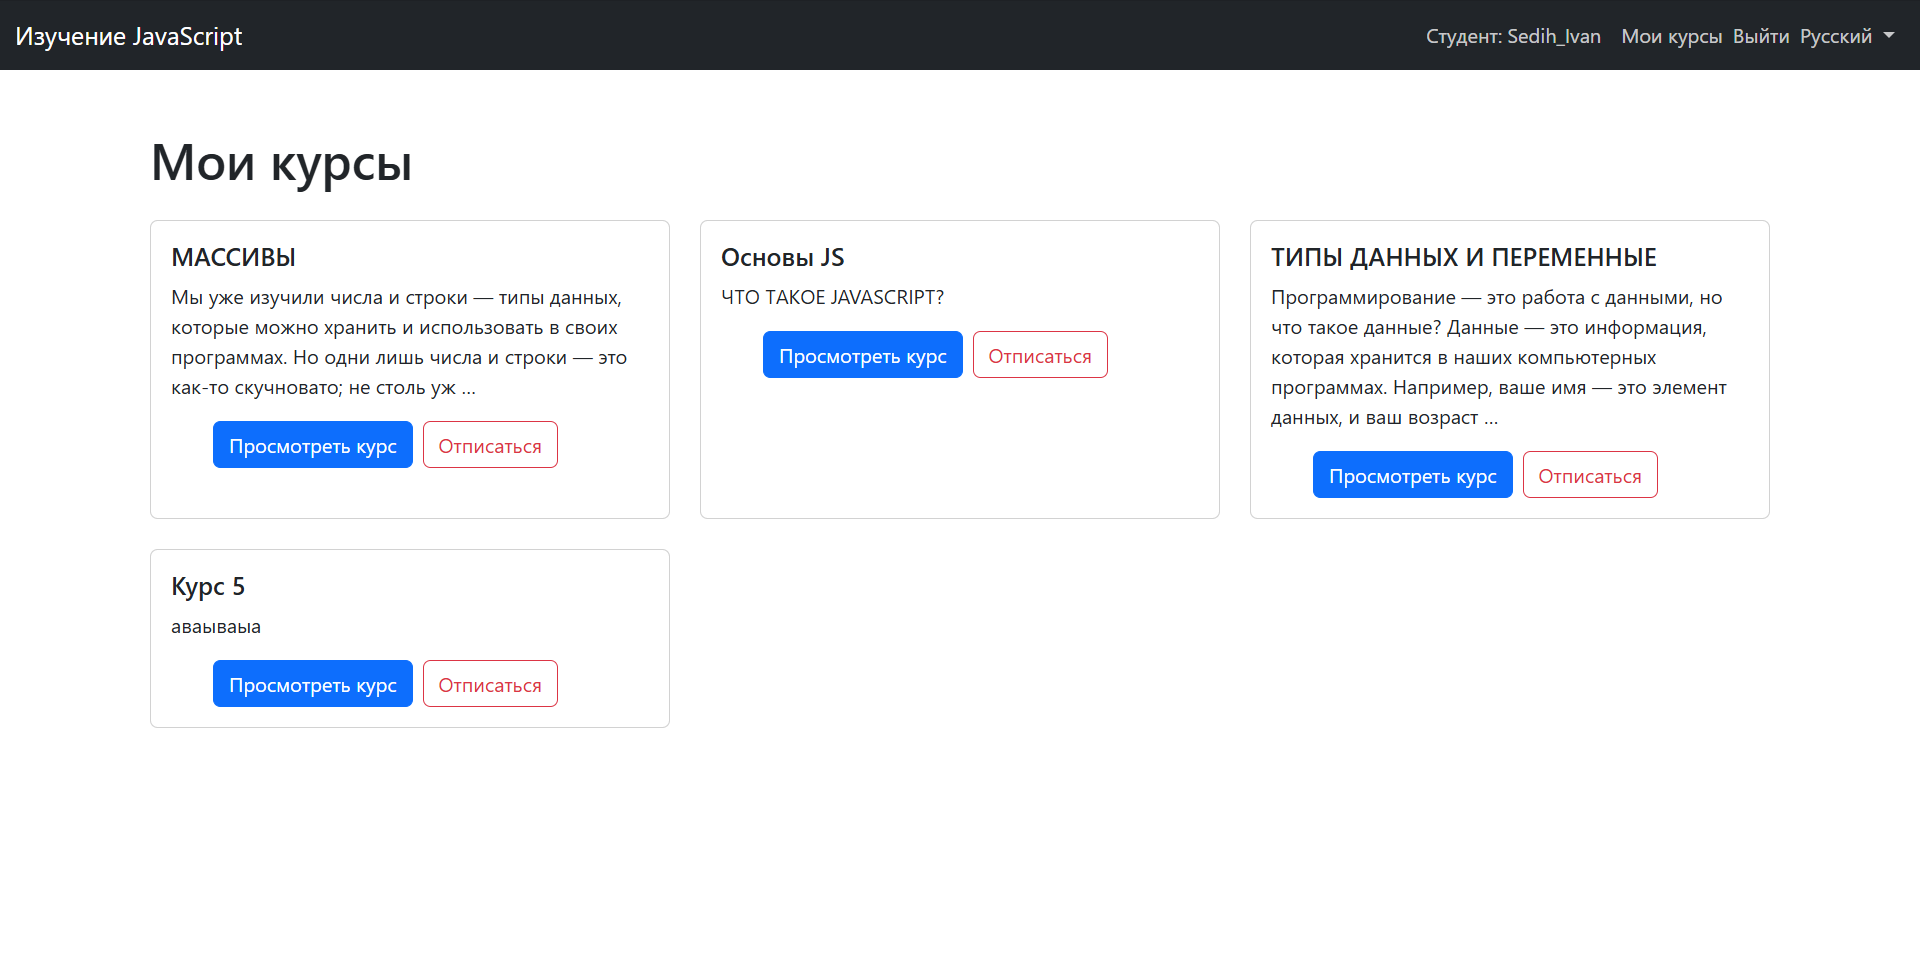
\includegraphics[width=0.8\linewidth]{images/профиль}
	\caption{Композиция интерфейса сервиса <<Профиль>>}
	\label{templ:image8}
\end{figure}
\newpage
\subsection*{Композиция шаблона создание курса представлена на рисунке ~\ref{templ:image9} и состоит из:}

\begin{itemize}
	\item окно создания курса (1);
	\item поле ввода заголовка курса (2);
	\item поле ввода описания курса (3);
	\item кнопка выбора изображения (4);
	\item поле выбора статуса курса (5);
	\item кнопка сохранения курса (6);
	\item кнопка отмены создания курса (7).
\end{itemize}

\begin{figure}[htp!]
	\centering
	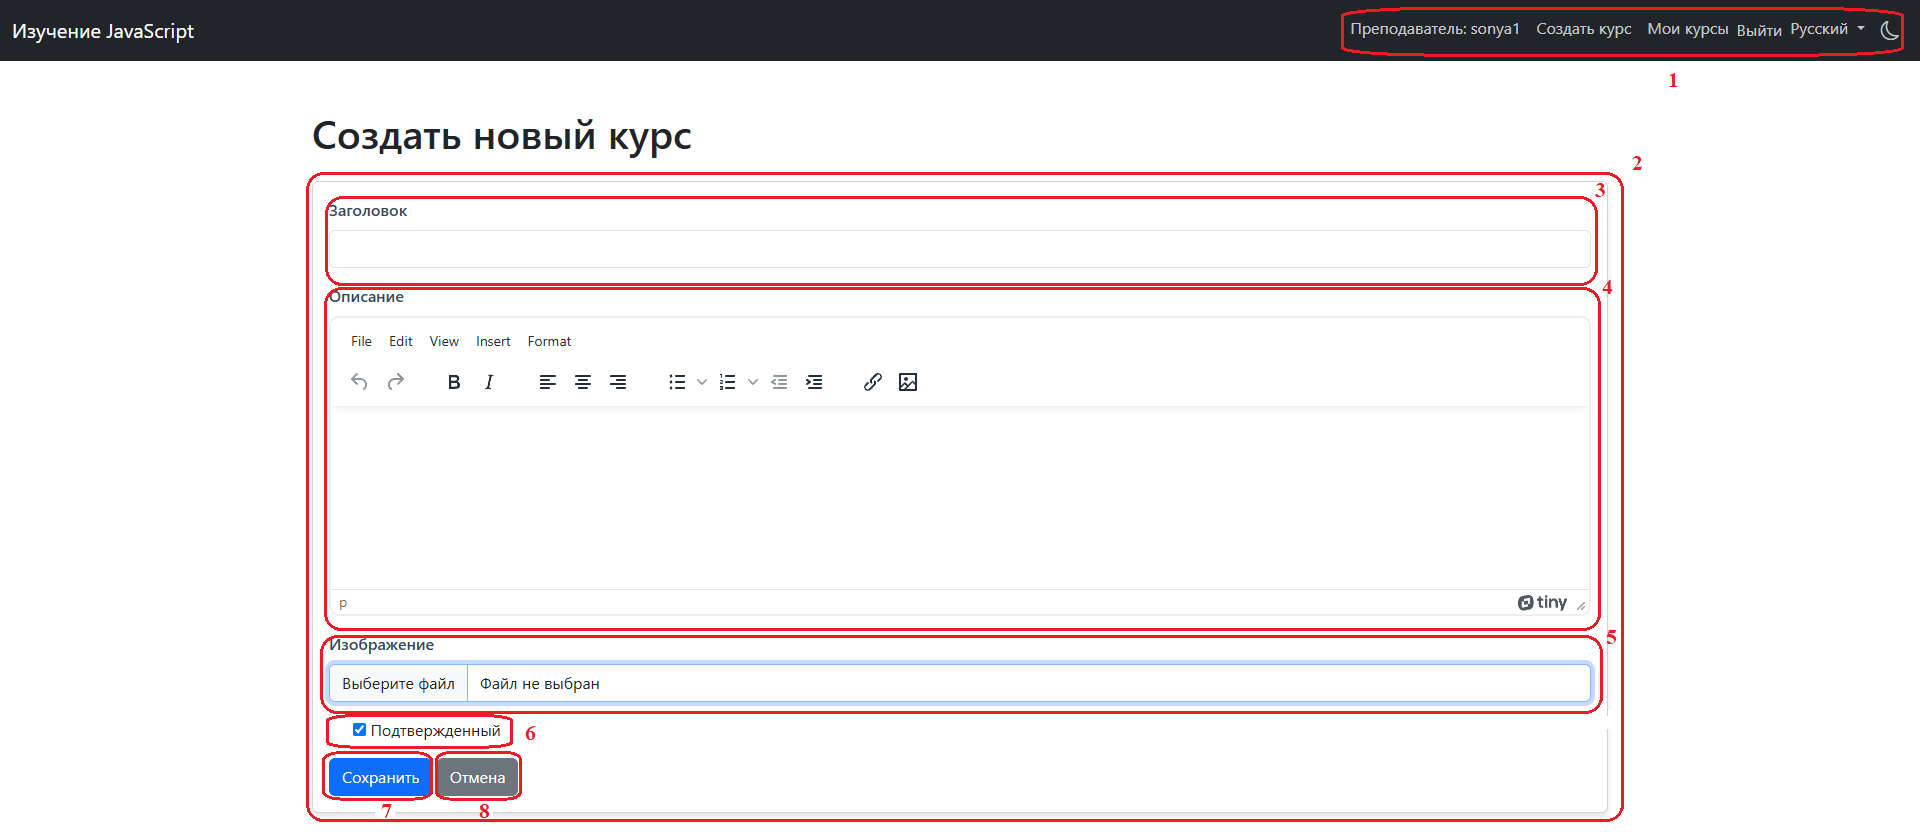
\includegraphics[width=0.8\linewidth]{images/создатькурс}
	\caption{Композиция интерфейса сервиса <<Создание курса>>}
	\label{templ:image9}
\end{figure}

\subsection*{Композиция шаблона создание урока представлена на рисунке ~\ref{templ:image10} и состоит из:}

\begin{itemize}
	\item окно создания урока (1);
	\item поле ввода заголовка урока (2);
	\item поле ввода описания урока (3);
	\item поле ввода материалов урока (4);
	\item поле ввода ссылки на видеоролик (5);
	\item поле выбора статуса урока (6);
	\item кнопка добавления урока (7).
\end{itemize}

\begin{figure}[htp!]
	\centering
	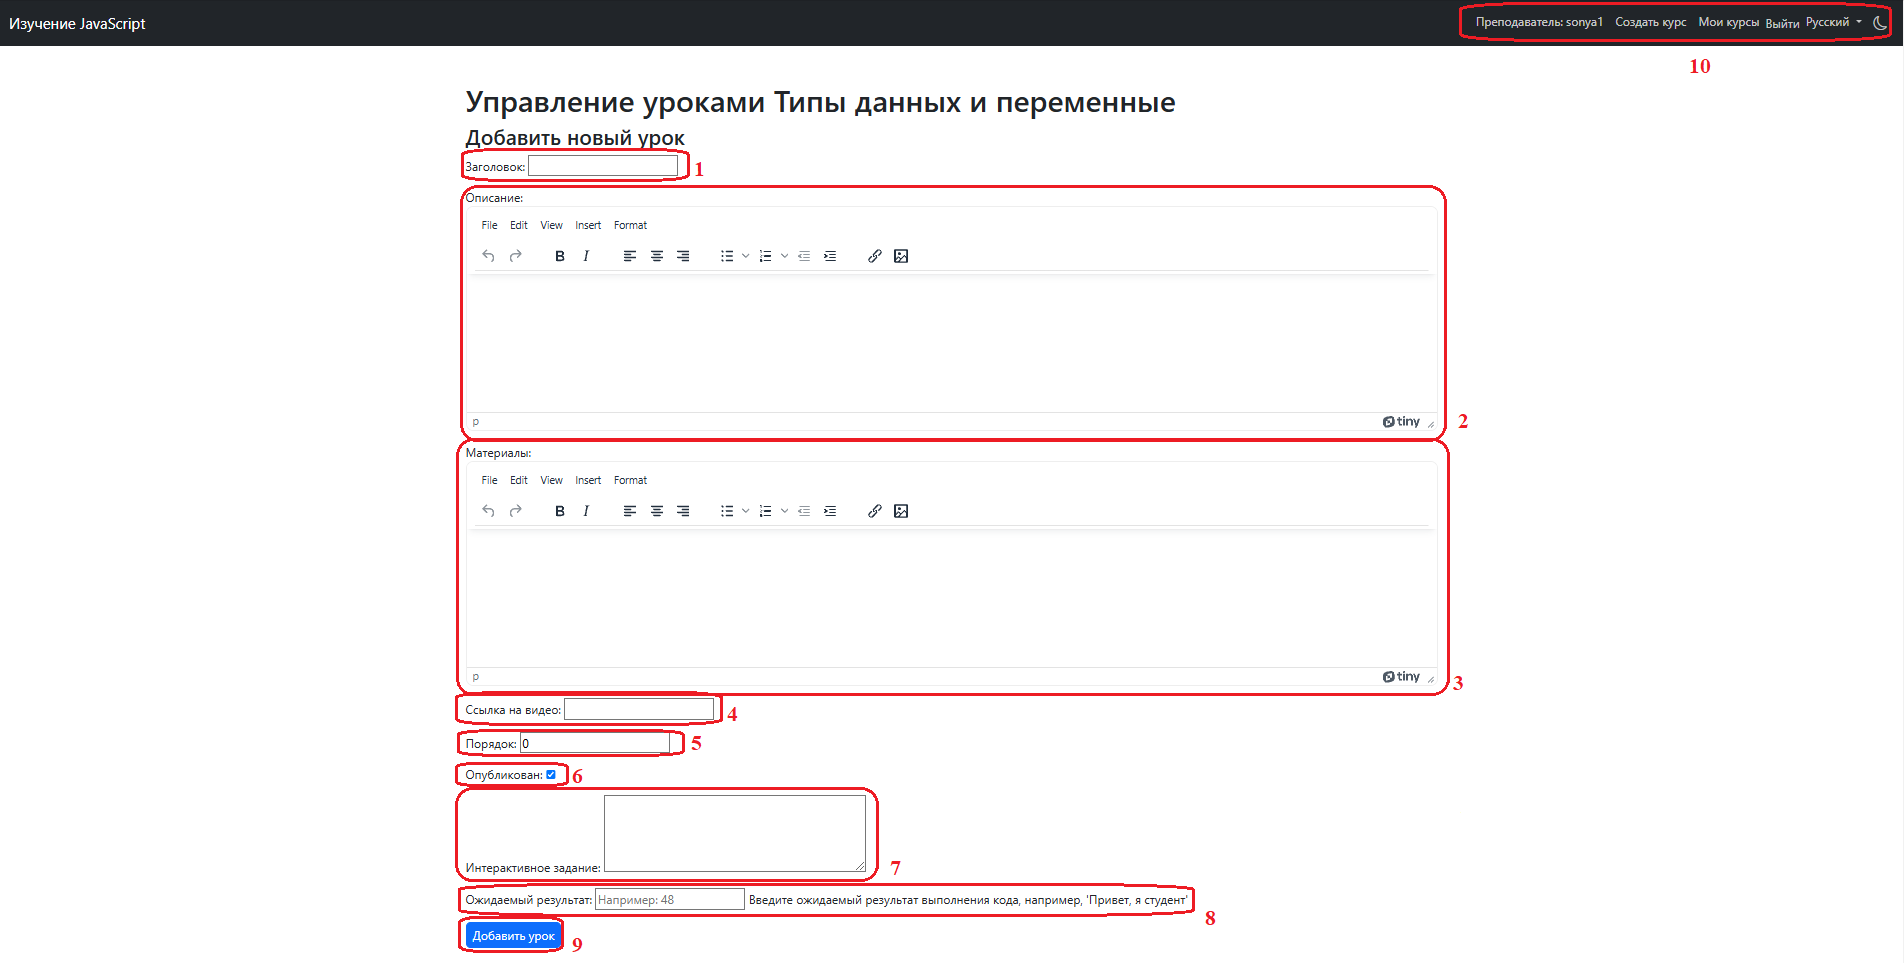
\includegraphics[width=0.8\linewidth]{images/создатьурок}
	\caption{Композиция интерфейса сервиса <<Создание урока>>}
	\label{templ:image10}
\end{figure}

\clearpage
\subsection{Моделирование вариантов использования}

Для разработки платформы была построена UML-диаграмма вариантов использования, отражающая взаимодействие пользователей с системой.

\begin{figure}[ht]
	\center{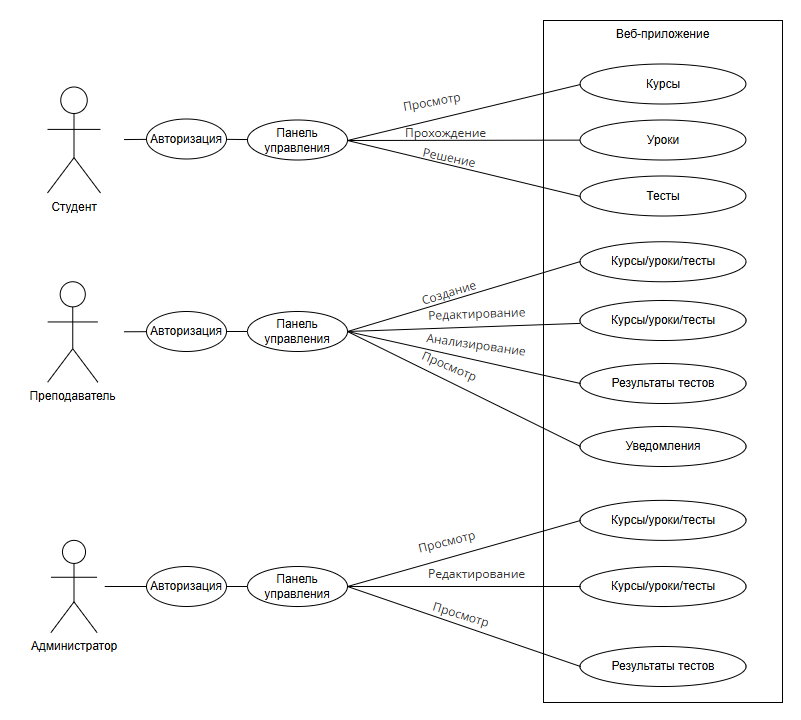
\includegraphics[width=0.9\linewidth]{images/UML}}
	\caption{Диаграмма прецедентов}
	\label{comp:image}
\end{figure}

Основные прецеденты системы:
\begin{itemize}
\item Авторизация и выход из системы.
\item Управление курсами.
\item Управление уроками.
\item Создание и управление тестами.
\item Прохождение тестов.
\item Просмотр результатов тестов.
\item Локализация интерфейса.

\end{itemize}


После авторизации в веб-платформе пользователь переходит на главную рабочую страницу <<панель управления для преподавателей или список курсов для студентов>>,  где отображаются доступные модули.

\begin{enumerate}
	\item Сервис <<Курсы>> — позволяет преподавателям создавать, редактировать и удалять курсы, а студентам --- просматривать доступные курсы и записываться на них. В сервисе отображается список курсов с кратким описанием и статусом (например, доступен или завершён).
	
	\item Сервис <<Уроки>> — предоставляет преподавателям возможность добавлять, редактировать и сортировать уроки в рамках курса. Студенты могут изучать материалы уроков (текст, изображения, видео). Сервис поддерживает предпросмотр уроков для преподавателей.
	
	\item Сервис <<Тесты>> — позволяет преподавателям создавать тесты с вопросами и вариантами ответов. Студенты проходят тесты, получая автоматическую оценку. Сервис интегрирован с модулем результатов для отслеживания успеваемости.
	
	\item Сервис <<Результаты тестов>> — предоставляет преподавателям инструменты для просмотра, анализа и удаления результатов тестов. Студенты могут видеть свои баллы и статистику по попыткам.
	
	\item Сервис <<Локализация>> — позволяет пользователям переключать язык интерфейса (например, русский, английский), что упрощает использование платформы для иностранных студентов. Поддерживается через Django-теги.
	
	\item Сервис <<Уведомления>> — отображает сообщения об успешных действиях (например, добавление урока, удаление результатов) или ошибках.
	
	\item Сервис <<Панель управления>> — главная страница для преподавателей, содержащая виджеты для быстрого доступа к курсам, урокам, тестам и результатам. Для студентов отображается список доступных курсов.
	
\end{enumerate}

\subsection{Требования к оформлению документации}

Разработка программной документации и программного изделия должна производиться согласно ГОСТ 19.102–77 и ГОСТ 34.601–90. Единая система программной документации.
